\documentclass{article}
%\documentclass[12pt]{article}
\usepackage[margin=1.5in]{geometry}     
%\usepackage[onehalfspacing]{setspace}
%\usepackage[doublespacing]{setspace}
\usepackage{amsmath, amssymb, amsthm}
\newtheorem{prop}{Proposition}
\usepackage{enumerate, enumitem}
\usepackage{bbm}
\usepackage{multirow}
\usepackage{booktabs}
\usepackage[utf8]{inputenc}
\usepackage{graphicx}
\usepackage[export]{adjustbox}
\usepackage{xcolor}
\usepackage{diagbox}
\usepackage{mathtools}
\usepackage{authblk}
\usepackage{parskip}
\def\Let@{\def\\{\notag\math@cr}}
\makeatother

\title{Optimal Carbon tax and Energy Substitution}
\author{Emmanuel Murray Leclair}
\affil{Department of Economics, Western University}
\date{August 2021}

\begin{document}
\nocite{*}

\maketitle

\section{Model}

\subsection{Framework}

The model to study energy input substitution is very similar to Acemoglu and Restrepo (2021) which I adapt to the energy market and augment it with costly switching. It features the assignment of a mix of energy inputs to energy tasks which allows for flexible variation in input usage, both at the extensive and intensive margin which is characteristic of data on fuel consumption the plant-level. I first present the structure of production for a given plant in a static setting, and then consider what happens when a new fuel can be added to the mix in a dynamic setting. There are two levels to production which correspond to two CES nests. The outer nest is standard and features typical TFP z, labor (l), capital (k), intermediates (m) and energy (E) inputs:

\begin{align}
    y &= z\Big( \alpha_k k^{\frac{\sigma-1}{\sigma}} + \alpha_l l^{\frac{\sigma-1}{\sigma}} + \alpha_m m^{\frac{\sigma-1}{\sigma}} + \alpha_e E^{\frac{\sigma-1}{\sigma}}\Big)^{\frac{\sigma}{\sigma-1}} \\
    \notag &\alpha_k + \alpha_l + \alpha_m + \alpha_e = 1
\end{align}

Where $\sigma \geq 0$ is the elasticity of substitution between inputs. The inner nest that composes E features a mass of M energy tasks in the $\omega \in (0,1)$ interval:

\begin{align}
    E = \Big( \frac{1}{M} \int_{0}^1 (M\tau(\omega))^{(\lambda-1)/\lambda} d \omega \Big)^{\lambda/(\lambda-1)}
\end{align}

I assume that tasks are gross complements, $\lambda \in (0,1)$, which will be motivated with specific examples. Each energy task can $\tau(\omega)$ and can be performed with a set of fuels $\{e_f\}_{f=1}^F$ (oil, gas, coal, electricity, etc.) which are in principle perfect substitutes:

\begin{align}
    \tau(\omega) = \sum_{f} \psi_f(\omega) e_f
\end{align}

Where $\psi_f(\omega)$ are fuel-by-task specific productivity terms, which are an important distinction from standard task-based production models and will allow for very flexible input usage. to motivate this framework one should be thinking of tasks such as the steps required to produce crude steel: preparation of raw material, conversion of iron ore into iron, and conversion of iron into crude steel (Luh et al. 2020). The preparation of raw materials typically requires coal whereas the two subsequent steps can be done with different fuels and the $\psi_f(\omega)$ terms can reflect these particularities. Moreover, these steps are complementary and require high amounts of energy.

Going back to the model, the inner nest problem can be solved in two steps: 

\begin{enumerate}
    \item Find the cheapest fuel to perform each task (section 1.2 and 1.3)
    \item Aggregate across tasks into fuel categories to get fuel demand (section 1.4).
\end{enumerate}

\subsection{Task choices: } Minimize the cost of producing one unit of energy E given task prices $p(\omega)$

\begin{align*}
    &\min_{\tau(\omega)} \Big\{ \int p(\omega) \tau(\omega) d\omega \Big\} \\
    s.t. \text{  }  E &= \Big( \frac{1}{M} \int_0^1 (M\tau(\omega))^{(\lambda-1)/\lambda} d\omega \Big)^{\lambda/(\lambda-1)} 
\end{align*}

This leads to demand for task $\omega$:

\begin{align}
    \tau(\omega)^* = \frac{E}{M} \Big( \frac{p_{\tau}}{p(\omega)} \Big)^{\lambda}
\end{align}

Where $p_{\tau}$ is the price index of energy tasks: 

\begin{align}
    p_{\tau} = \Big(  \int_0^1 p(\omega)^{1-\lambda} M d\omega \Big)^{1/(1-\lambda)}
\end{align}

\subsection{Assignment of fuels to energy tasks: } 

To study the assignment of fuels to task with costly switching, I need to define a reference set of fuels available to the plant (which will the set of fuels used last period in the dynamic model) $\mathcal{F}$ which defines the set of tasks that were performed by fuel f in the reference distribution. For now, I shall present the assignment of fuels to energy tasks given $\mathcal{F}$. A plant finds the fuel that minimize the cost of performing task $\omega$ given (exogenous) fuel prices:

\begin{align*}
    &\min_{\{e_f(\omega)\}_{f \in \mathcal{F}}} \sum_{f \in \mathcal{F}} p_f e_f(\omega) \\
    s.t. &\text{   } \sum_{f \in \mathcal{F} } \psi_f(\omega) e_f(\omega) = \tau(\omega)
\end{align*}

By the linearity of this problem implied by perfect substitution, the plant chooses the fuel that has the lowest unit cost to produce the task. Hence, task prices follow:

\begin{align}
    p(\omega) = \min \Big\{ \frac{p_1}{ \psi_1(\omega)},...,\frac{p_F}{\psi_F(\omega)} \Big\}
\end{align}

This set-up has one important implications. The fuel-by-task productivity terms will play an important role to determine the energy efficiency of different fuels. For example, since natural gas is consistently more expensive than coal and oil in India, only plants with large productivity draws for natural gas will use it, and if tasks are gross complements ($\lambda < 1$) the quantity consumed will be decreasing in its productivity, making natural gas more energy efficient as observed in the data\footnote{proof in appendix}.

\subsection{Aggregation from tasks to fuels}

From the problem before, I can define the set of tasks that are performed by each fuel:

\begin{align}
    \mathcal{T}_f = \Big\{ \omega: \frac{p_f}{\psi_f(\omega)} \leq \frac{p_j}{\psi_j(\omega)} \forall j \neq f  \Big\}
\end{align}

Then, I can redefine the aggregate price index of energy tasks in (5):

\begin{align}
    p_{\tau} = \Bigg( \sum_{f \in \mathcal{F}} p_f^{1-\lambda} M \int_{\mathcal{T}_f} \psi_f(\omega)^{\lambda-1} d\omega \Bigg)^{1/(1-\lambda)}
\end{align}

Notice that the price index of energy tasks is the same as the price of the aggregate energy input E:

\begin{align*}
    p_e E &= \int_0^1 \tau(\omega) p(\omega) d\omega \\
    p_e E &= E \int_0^1 \Big( \frac{p_{\tau}}{p(\omega)} \Big)^{\lambda} p(\omega) d\omega \\
    p_e &= p_{\tau}^{\lambda} \int_0^1 p(\omega)^{1-\lambda} d\omega \\
    p_e &= p_{\tau}^{\lambda} p_{\tau}^{1-\lambda} \\
    p_e &= p_{\tau}
\end{align*}

This has important implications. It means fuel choices are such that they minimizes the effective price of energy $p_e$. Hence, expanding $\mathcal{F}$ to $\mathcal{F'}$ by adding a new fuel will serve to expand the choice set in the minimization problem of (6) and allow the plant to face a weakly lower price of energy. Moreover, it means that all the heterogeneity from the fuel-by-task productivity terms is captured by a single term, $p_e$. I can now define the demand for a task performed by fuel f from (4):

\begin{align}
    \tau_f(\omega) = \frac{E}{M} \Big( \frac{ \psi_f(\omega)}{p_f} p_e \Big)^{\lambda}
\end{align}

Using the task production function from section 1.1, I can find the conditional demand for fuel f by equalizing (9) with (3) and integrating over all tasks performed by fuel f ($\mathcal{T}_f$):

\begin{align*}
     \psi_f(\omega) e_f(\omega) &= \frac{E}{M} \Big( \frac{ \psi_f(\omega)}{p_f} p_e \Big)^{\lambda} \\
    e_f(\omega) &= \frac{E}{M} \Big( \frac{p_e}{p_f} \Big)^{\lambda} \big(\psi_f(\omega) \big)^{\lambda-1}
\end{align*}

Then,

\begin{align}
    e_f &= E \Big( \frac{p_e}{p_f} \Big)^{\lambda} \underbrace{ \frac{1}{M} \int_{\mathcal{T}_f} \psi_f(\omega)^{\lambda-1} d\omega}_{\Gamma_f} \\
    &= E \Big( \frac{p_e}{p_f} \Big)^{\lambda} \Gamma_F
\end{align}

Where $\Gamma_f$ is referred to the task-share of energy input (fuel) f.

\textbf{I can now use this conditional fuel demand and the energy price index in (8) to back out the production function for E as a function of energy inputs:}

\begin{enumerate}
    \item Rearrange (10):
    \begin{align}
        p_f = \frac{E^{1/\lambda} P_e \Gamma_f^{1/\lambda}}  {e_f^{1/\lambda}}
    \end{align}
    \item plug (11) into (8) and solve for E:
    \begin{align}
        E = \Bigg( \sum_{f \in \mathcal{F}} \Gamma_f^{1/\lambda} \big( e_f \big)^{(\lambda-1)/\lambda} \Bigg)^{\lambda/(\lambda-1)}
    \end{align}
\end{enumerate}

The production function for energy in (12) looks like a standard CES in different energy inputs with a key distinction: the presence of $\Gamma_f$, the endogenous share of tasks performed by fuel f. This term can be 0 if a fuel is always dominated by at least one other fuel, or it can be 1 if this fuel always dominates every other fuels. This implies that the production function in (12) is very flexible and allows for corner solutions, a key feature of data on fossil fuel consumption.


\subsection{Solving for Optimal Energy Input Choices given $\mathcal{F}$}

Plants indexed by i are heterogeneous in fuel-by-task specific productivity ($\psi_{if}(\omega)$). Without loss of generality, I remove fuel-augmenting productivity terms ($A_f$) from the analysis as they are endogenously determined by the distribution of $\psi$'s across all tasks. In the first year of production, I assume that plants draw fuel-by-task productivity terms for each fuels and tasks from a fuel-specific Pareto distribution such that:

\begin{align*}
    P(\psi_{if}(\omega) \geq x) = \Big(\frac{x}{\gamma_f}\Big)^{-\alpha_f}
\end{align*}

Then, the probability fuel f is chosen over fuel j is:

\begin{align*}
    P_r\Big(\frac{p_f}{\psi_{if}(\omega)} \leq \frac{p_j}{\psi_{if}(\omega)}\Big) &= \Big( \frac{p_f}{p_j \gamma_f}\Big)^{-\alpha_f} \int_{\gamma_j}^{\infty} \psi_j^{-\alpha_f}f(\psi_j(\omega)) d\psi_j \\
    &= \Big( \frac{p_f}{p_j \gamma_f}\Big)^{-\alpha_f} \int_{\gamma_j}^{\infty} \psi_j^{-\alpha_f-\alpha_j-1} \alpha_j \gamma_j^{\alpha_j} d\psi_j \\
    &= \Big( \frac{p_f}{p_j \gamma_f}\Big)^{-\alpha_f} \Big[ \frac{\psi_j^{-\alpha_f-\alpha_j}}{-\alpha_f-\alpha_j} \alpha_j \gamma_j^{\alpha_j} \Big]_{\gamma_j}^{\infty} \\
    &= \Big( \frac{p_f}{p_j} \Big)^{-\alpha_f} \Big( \frac{\gamma_j}{\gamma_f} \Big)^{-\alpha_f} \frac{\alpha_j}{\alpha_f+\alpha_j}
\end{align*}

Then, if there are F number of fuels, the probability that fuel f is chosen over all other fuels to perform task $\omega$ is going to be:

\begin{align}
    \tau_f(\omega) &=  \prod_{j \neq f} P_r\Big(\frac{p_f}{\psi_{if}(\omega)} \leq \frac{p_j}{\psi_{ij}(\omega)}\Big) \notag\\ 
    &= \Big( \frac{\gamma_f}{p_f} \Big)^{(F-1)\alpha_f} \prod_{j \neq f} \Big( \frac{\gamma_j}{p_j} \Big)^{-\alpha_f} \frac{\alpha_j}{\alpha_f + \alpha_j} = \tau_f
\end{align}

If there are M tasks, I can define the probability that a given fuel is used m times which follows a binomial distribution. Let $M \mathcal{T}_f$ be the number of times fuel f is chosen:

\begin{align}
    P_r(M \mathcal{T}_f = m) =  \Big( \frac{M}{m} \Big)\tau_f^{m}(1-\tau_f)^{M-m}
\end{align}

Where $\big( \frac{M}{m} \big) = \frac{M!}{m!(M-m)!}$. Notice that by the Poisson Limit Theorem, the limiting distribution (as $M \rightarrow \infty$) only exist for $m < M$. This assumption is used extensively in the literature on technological choices (\textbf{Kortum 1997, Buera and Oberfield 2020, Boehm and Oberfield 2020}). However, in my context it means there can not be any corner solution where a fuel is used for all tasks if the number of tasks goes to infinity. For this reasons, I keep the assumption of a finite number of tasks for the remainder of the paper.

With (15) I can now characterize the distribution of fuel shares, which is going to be continuous because productivity draws affect how much fuel is consumed. For example, when tasks are gross complement ($\lambda < 1$) a lower quantity of fuel is going to be needed if it is very productive and vice versa. For a given plant, let fuel shares be:

\begin{align}
    s_{f} &= \frac{e_{f}}{\sum_f e_{f}} \notag\\
    &= \frac{p_f^{-\lambda} \Gamma_{f}}{\sum_f p_f^{-\lambda} \Gamma_{f}}
\end{align}

\textit{First moment (mean)}

Notice that with M tasks and a probability of success $\tau_f$ the average number of times fuel f is chosen in the data is going to be:

\begin{align*}
    E(M \mathcal{T}_f) = M \tau_f \\
    E(\mathcal{T}_f)  = \tau_f
\end{align*}

Then, I can use that to characterize $E(\Gamma_f)$ and $E(s_f)$:`

\begin{align*}
    E(\Gamma_f) &= E\Big( \frac{1}{M} \int_{\mathcal{T}_f} \psi_f(\omega)^{\lambda-1} d\omega \Big) \\
    &= ???
\end{align*}

\subsection{Full model and expanding fuel set $\mathcal{F}$}

Each period there is a representative consumer with exogenous income $I_t$ who consumes a final good $Y_t$ with price $P_t$:

\begin{align*}
    P_t Y_t = I_t \\
    Y_t = \frac{I_t}{P_t}
\end{align*}

To form the final good Y, there is a continuum of plants who produce differentiated goods index by $\varphi$ that can be substituted at rate $\rho > 1$, which can be extended to include multiple industries later on:

\begin{align}
    Y_t = \Big( \int_0^1 y_t(\varphi)^{\frac{\rho}{\rho-1}} dF(\varphi)  \Big)^{\frac{\rho}{\rho-1}}
\end{align}

Each differentiated good (plant) faces then faces inverse demand:

\begin{align}
    p_t(\varphi) = \Big( \frac{I_t}{y_t(\varphi)}\Big)^{\frac{1}{\rho}} P_t^{\frac{\rho}{\rho-1}}
\end{align}

At the beginning of each period a given plant observes the set of fuels available today $\mathcal{F}_t$, the set of fuel-by-task productivity $\Psi_t \in \mathbb{R}^{M x \mathcal{F}_t}$ and fuel prices $p_{ft}$, and it solves the static problem of allocating fuels to tasks, which gives each plant its price of energy $p_{et}(\Psi_t,\mathcal{F}_t)$ from (8) and its pollution intensity of energy, which will be useful later for characterizing optimal policy. The plant then observes its total factor productivity $z_t$, the fixed cost of expanding $\mathcal{F}_t$ by one fuel $\kappa$, capital $k_t$ and input prices $w_t,p_{mt}, r_{t}$. It then chooses flexible inputs today $l_t,m_t,E_t$, capital next year $k_{t+1}$ and the set of fuels available for next year to maximize the following value function: 
\begin{multline}
    V_t(k_t,z_t,\Psi_t,\mathcal{F}_t) = \max_{k_{t+1},l_t,m_t,E_t,\mathcal{F}_{t+1}}I_t^{\frac{1}{\rho}} (P_t y_t(\varphi))^{\frac{\rho-1}{\rho}} - w_t l_t - p_{mt}m_t - r_{t}k_{t+1} - p_e(\Psi_t,\mathcal{F}_t) \\ -\mathbb{I}(\mathcal{F}_{t+1} > \mathcal{F}_t)
    + \beta E_t V_{t+1}(k_{t+1},z_{t+1},\Psi_{t+1},\mathcal{F}_{t+1})
\end{multline}

\begin{align*}
    \text{s.t.  }     y_t(\varphi) &= z_t\Big( \alpha_k k_t^{\frac{\sigma-1}{\sigma}} + \alpha_l l_t^{\frac{\sigma-1}{\sigma}} + \alpha_m m_t^{\frac{\sigma-1}{\sigma}} + \alpha_e E_t^{\frac{\sigma-1}{\sigma}}\Big)^{\frac{\sigma}{\sigma-1}}
\end{align*}

I also assume that fuel-by-task productivity terms follow a unit root process, which means plants expected to get the same productivity draws tomorrow as the ones they observe today for fuels in $\mathcal{F}_t$, whereas they take expectation over the cross-sectional distribution of productivity for fuels that are not yet in $\mathcal{F}_t$. This has the implication that the allocation of fuels to tasks carries no dynamic implications. For example, if a plant doesn't use a fuel that is in $\mathcal{F}_t$ because it got bad productivity draws for that fuel, it drops from $\mathcal{F}_{t+1}$. However, if the plant expects to get the same productivity next period, it also expect not to use that fuel next period. \textbf{Need to show this formally (I want $E(p_e(\Psi_{t+1},\mathcal{F}_t)|\Psi_t) = E(p_e(\Psi_t,\mathcal{F}_t))$}. 

\begin{align*}
    \psi_{f,t+1}(\omega) &= \psi_{ft}(\omega) + \epsilon_{f,t+1}(\omega) \\
    \psi_{f,t+1} &= \psi_{ft} + \epsilon_{f,t+1} \text{  by symmetry of tasks}
\end{align*}

Where $E(\epsilon_{f,t+1}) = 0$. For now, I also assume that plants can only increase the set of fuels by one fuel. To get some intuition, it is useful to see this problem with a timeline:

\begin{figure}[htp]
    \centering
    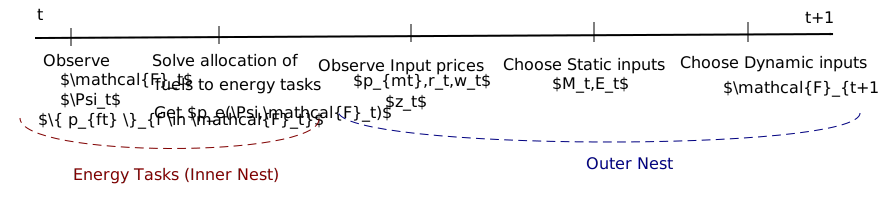
\includegraphics[width=\linewidth]{timeline.pdf}
    \caption{timeline of production decisions}
    \label{fig:my_label}
\end{figure}

\begin{prop}
    Larger (more productive) plants are more likely to add a new fuel to the mix
\end{prop}





\subsection{Adding a new fuel in a dynamic setting (preliminary)}

Let us now consider the problem of a firm that wants to add a new fuel to its fuel mix $\mathcal{F}$. It pays a fixed cost $\kappa$ today and have access to this new fuel next period and all subsequent periods. For example, one can think of a firm located away from gas pipelines considering the inclusion of natural gas to its mix. It may need to transport liquefied natural gas (LNG) and install its own compressors/vaporizers to turn the liquid back into a gas which is a significant investment. The value function of a firm takes capital today, a vector of technology/productivity terms ($\mathcal{Z} = \{A_f\}, \{ \psi_f(\omega) \},z)$ which are assumed to evolve stochastically and the set of energy inputs/fuels available to the firm $\mathcal{F}$:

\begin{align*}
    \mathcal{V}(k,\mathcal{Z},\mathcal{F}) &= P z \Big( l^{\frac{\sigma-1}{\sigma}} + k^{\frac{\sigma-1}{\sigma}} + m^{\frac{\sigma-1}{\sigma}} + E^{\frac{\sigma-1}{\sigma}}\Big)^{\frac{\sigma}{\sigma-1}} \\ 
    & - wl - p_m m - r_k k - p_e(\mathcal{F},\mathcal{Z}) E - \sum_f\kappa_f \mathbb{I}(e_f \in \mathcal{F'} \setminus \mathcal{F}) + \beta \mathbb{E}_{x \in \mathcal{Z}} \mathcal{V}(k',\mathcal{Z'},\mathcal{F'})
\end{align*}

Where $p_e(\mathcal{F},\mathcal{Z})$ is given when solving:

\begin{align*}
    \min_{\{e_f\}_{f \in \mathcal{F}}} &\sum_{f \in \mathcal{F}} p_f e_f \\
    s.t. \text{   } E &= \Bigg( \sum_{f \in F} \Gamma_f(\mathcal{Z})^{1/\lambda} \big( A_f e_f \big)^{(\lambda-1)/\lambda} \Bigg)^{\lambda/(\lambda-1)} 
\end{align*}

\subsection{Solving for Optimal Energy Input Choices - Initial year Static}

Plants indexed by i are heterogeneous in fuel-by-task specific productivity ($\psi_{if}(\omega)$). Without loss of generality, I remove fuel-augmenting productivity terms ($A_f$) from the analysis as they are endogenously determined by the distribution of $\psi$'s across all tasks. In the first year of production, I assume that plants draw fuel-by-task productivity terms for each fuels and tasks from a fuel-specific Pareto distribution such that:

\begin{align*}
    P(\psi_{if}(\omega) \geq x) = \Big(\frac{x}{\gamma_f}\Big)^{-\alpha_f}
\end{align*}

Then, the probability fuel f is chosen over fuel j is:

\begin{align*}
    P_r\Big(\frac{p_f}{\psi_{if}(\omega)} \leq \frac{p_j}{\psi_{if}(\omega)}\Big) &= \Big( \frac{p_f}{p_j \gamma_f}\Big)^{-\alpha_f} \int_{\gamma_j}^{\infty} \psi_j^{-\alpha_f}f(\psi_j(\omega)) d\psi_j \\
    &= \Big( \frac{p_f}{p_j \gamma_f}\Big)^{-\alpha_f} \int_{\gamma_j}^{\infty} \psi_j^{-\alpha_f-\alpha_j-1} \alpha_j \gamma_j^{\alpha_j} d\psi_j \\
    &= \Big( \frac{p_f}{p_j \gamma_f}\Big)^{-\alpha_f} \Big[ \frac{\psi_j^{-\alpha_f-\alpha_j}}{-\alpha_f-\alpha_j} \alpha_j \gamma_j^{\alpha_j} \Big]_{\gamma_j}^{\infty} \\
    &= \Big( \frac{p_f}{p_j} \Big)^{-\alpha_f} \Big( \frac{\gamma_j}{\gamma_f} \Big)^{-\alpha_f} \frac{\alpha_j}{\alpha_f+\alpha_j}
\end{align*}

Then, if there are F number of fuels, the probability that fuel f is chosen over all other fuels to perform task $\omega$ is going to be:

\begin{align}
    \tau_f(\omega) &=  \prod_{j \neq f} P_r\Big(\frac{p_f}{\psi_{if}(\omega)} \leq \frac{p_j}{\psi_{ij}(\omega)}\Big) \notag\\ 
    &= \Big( \frac{\gamma_f}{p_f} \Big)^{(F-1)\alpha_f} \prod_{j \neq f} \Big( \frac{\gamma_j}{p_j} \Big)^{-\alpha_f} \frac{\alpha_j}{\alpha_f + \alpha_j} = \tau_f
\end{align}

If there are M tasks, I can define the probability that a given fuel is used m times which follows a binomial distribution. Let $M \mathcal{T}_f$ be the number of times fuel f is chosen:

\begin{align}
    P_r(M \mathcal{T}_f = m) =  \Big( \frac{M}{m} \Big)\tau_f^{m}(1-\tau_f)^{M-m}
\end{align}

Where $\big( \frac{M}{m} \big) = \frac{M!}{m!(M-m)!}$. Notice that by the Poisson Limit Theorem, the limiting distribution (as $M \rightarrow \infty$) only exist for $m < M$. This assumption is used extensively in the literature on technological choices (\textbf{Kortum 1997, Buera and Oberfield 2020, Boehm and Oberfield 2020}). However, in my context it means there can not be any corner solution where a fuel is used for all tasks if the number of tasks goes to infinity. For this reasons, I keep the assumption of a finite number of tasks for the remainder of the paper.

With (15) I can now characterize the distribution of fuel shares, which is going to be continuous because productivity draws affect how much fuel is consumed. For example, when tasks are gross complement ($\lambda < 1$) a lower quantity of fuel is going to be needed if it is very productive and vice versa. For a given plant, let fuel shares be:

\begin{align}
    s_{f} &= \frac{e_{f}}{\sum_f e_{f}} \notag\\
    &= \frac{p_f^{-\lambda} \Gamma_{f}}{\sum_f p_f^{-\lambda} \Gamma_{f}}
\end{align}

\textit{First moment (mean)}

Notice that with M tasks and a probability of success $\tau_f$ the average number of times fuel f is chosen in the data is going to be:

\begin{align*}
    E(M \mathcal{T}_f) = M \tau_f \\
    E(\mathcal{T}_f)  = \tau_f
\end{align*}

Then, I can use that to characterize $E(\Gamma_f)$ and $E(s_f)$:`

\begin{align*}
    E(\Gamma_f) &= E\Big( \frac{1}{M} \int_{\mathcal{T}_f} \psi_f(\omega)^{\lambda-1} d\omega \Big) \\
    &= ???
\end{align*}

\end{document}
